\section*{Dati e risultati}









%\begin{wrapfloat}{figure}{O}{0pt}
%        \def\svgwidth{0.4\textwidth}
%        \subimport{figure/}{raddrizzatore.pdf_tex}
%        \caption{Raddrizzatore di precisione a semionda. Alimentato, inizialmente con una $V\ped{in}\,=\,\SI{1.02}{\volt}$ di frequenza $\nu\,=\,\SI{50}{\hertz}$.}
%        \label{fig:radd}
%\end{wrapfloat}

%\begin{SCfigure}[][p]
%        \centering
%        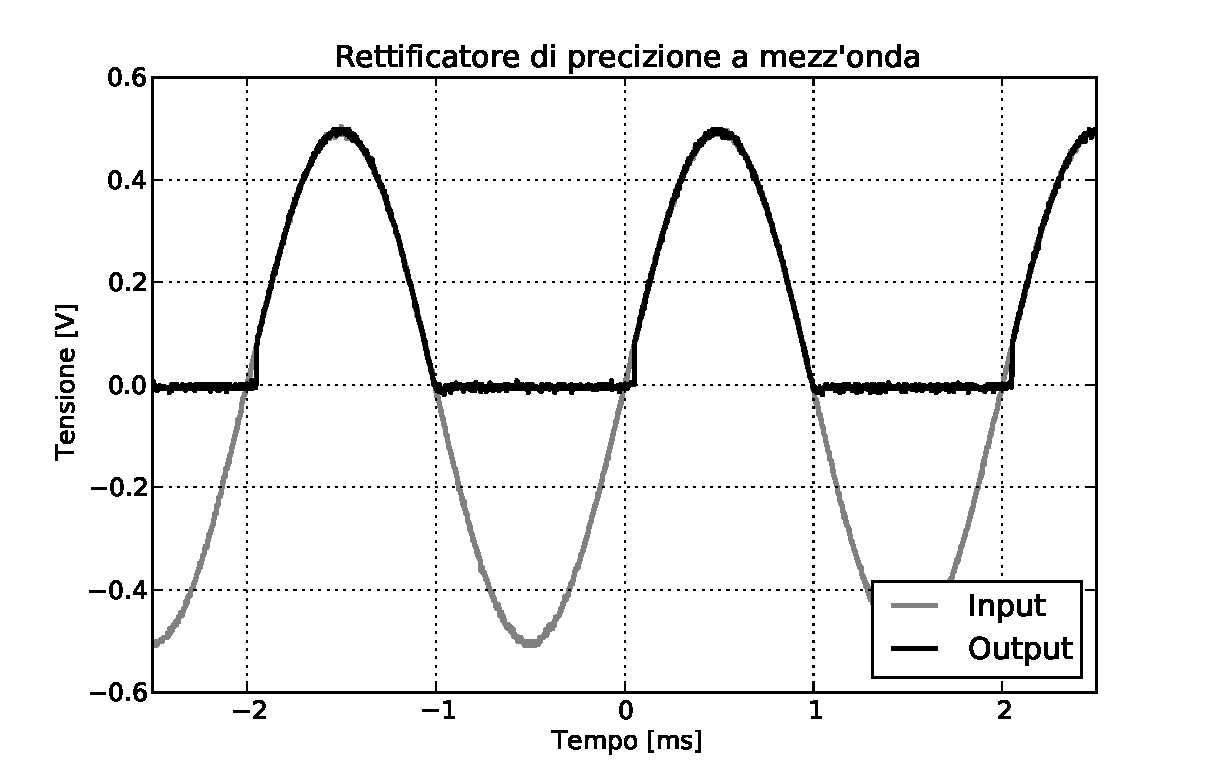
\includegraphics[width=0.7\textwidth]{figure/rett.pdf}
%        \caption{Questo grafico illustra l'andamento di $V\ped{out}$, linea nera, in funzione di $V\ped{in}$, linea grigia. Si nota chiaramente, come da previsioni, che la parte negativa del segnale in ingresso impediscse al diodo di condurre, pertanto la tensione di output risulta nulla. Inoltre, come si può osservare, il fronte di salita di $V\ped{out}$ presenta un leggero ritardo rispetto al segnale in ingresso $V\ped{in}$. Questo ritardo è stato stimato essere approssimativamente di circa $(152\pm10)\SI{}{\micro\second}$.}
%        \label{fig:radd_plot1}
%\end{SCfigure}
